\documentclass[12pt]{article}
\usepackage[a4paper]{geometry}
\usepackage[pdftex]{hyperref}
\usepackage[german]{babel}
\usepackage[utf8]{inputenc}
\usepackage{csquotes}
\usepackage{amssymb}
\usepackage{graphicx}
\usepackage{multicol}
\usepackage{amsmath}
\usepackage{enumitem}
\usepackage{fancyhdr}
\usepackage{indentfirst}
\usepackage{polynom}

\geometry{
  headheight=14px,
  left=2.54cm,
  right=2.54cm,
  bottom=2cm,
  top=2cm
}

\setlength{\marginparsep}{1 cm}
\setlength{\topmargin}{-0.6in}
\setlength{\textheight}{9.5in}
\pagestyle{fancy}

% German-style quotation marks %
\MakeOuterQuote{"}

% Typesetting differential operator %
\providecommand\d{}
\renewcommand{\d}[1]{\:\mathrm{d}{#1}} 

\polyset{%
   style=C,
   delims={\big(}{\big)},
   div=:
}

\fancypagestyle{firstpage}{%
  \lhead{\bf Name:}
  \rhead{\bf Anzahl zusätzlicher Blätter:\space\space\space\space\space}
}

\begin{document}

\thispagestyle{firstpage}

\begin{center}
{\bf {\large Wiederholungsklausur Analysis (3IT18-1, 3MI18-1)}}
\end{center}

\begin{center}
\textbf {Der Rechengang muss eindeutig und vollständig ersichtlich sein!}
\end{center}

\textbf{Hilfsmittel}: Kein Taschenrechner, ein handbeschriebenes A4-Blatt.

\begin{center}
Bitte nutzen Sie nach Möglichkeit den Platz auf den Aufgabenblättern und den Rückseiten. Zusätzlich beschriebene Blätter heften Sie bitte an diese Klausur.
\end{center}

\section*{Bewertung}

\begin{itemize}
\item Aufgabe 1:      \space\space\space\space\space$/08$
\item Aufgabe 2:      \space\space\space\space\space$/07$
\item Aufgabe 3:      \space\space\space\space\space$/07$
\item Aufgabe 4:      \space\space\space\space\space$/08$
\item Zusatzaufgabe:  \space\space\space\space\space$/02$
\end{itemize}

\textbf{Gesamt}: \space\space\space\space\space %$/$

\begin{center}
{\bf {\large Viel Erfolg!}}
\end{center}

\newpage
\section* {Aufgabe 1}

\begin{center}
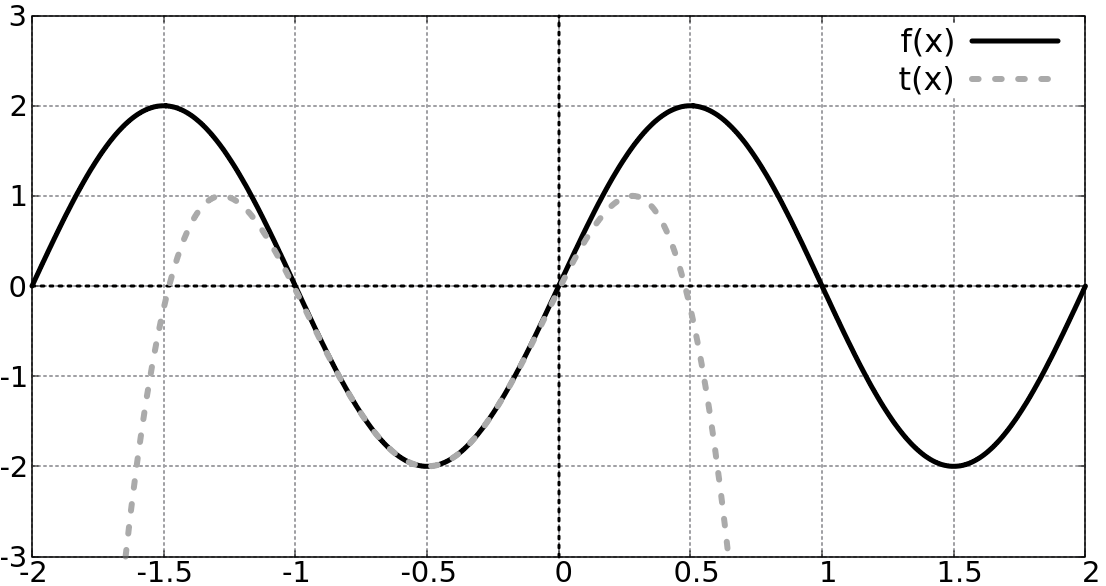
\includegraphics[width=0.95\textwidth]{grid_klausur.png}
\end{center}

\begin{enumerate}[label=(\alph*)]
\item (2P) In der oberen Skizze ist die Funktion $f(x)$ dargestellt. Es handelt sich um eine skalierte Sinusfunktion. Lesen Sie für $f(x)$ folgende Eigenschaften ab:
\begin{itemize}
\item Amplitude:
\item Periode:

\end{itemize}
\item (2P) Finden Sie für $f(x)$ eine mögliche Funktionsgleichung! \\
\\
$f(x)=$
\\

\item (4P) Weiterhin ist in der Skizze das Taylorpolynom $t(x)$ an die Funktion $f(x)$  eingezeichnet. Beantworten Sie anhand der Skizze:
\begin{itemize}
\item Wie lautet die Entwicklungsstelle $x_0$ für das Taylorpolynom $t$? \\
\\
\\

\item Der Grad des Taylorpolynoms $t$ beträgt wenigstens 4. Warum?\\
\\
\\

\item Was ist der größte Wert des Restglieds im Intervall $[-1{,}5;0{,}5]$? Tragen Sie diesen in der Skizze ein!
\end{itemize}
\end {enumerate}

\newpage
\section* {Aufgabe 2}

Für Polynome 2. Grads der Form $p_2(x)=x^2+ax+b = (x-r_1)(x-r_2)$ trifft der sogenannte "Satz von Vieta" die folgende \textbf{Aussage}:

\begin{align*}
&a = -(r_1+r_2)\\
&b= r_1r_2\\
\end{align*}

\begin{enumerate}[label=(\alph*)]

\item (4P) Welche (graphische) Bedeutung haben $r_1$ und $r_2$? Wie lauten $a$, $b$ und $r_1$ und $r_2$ für das Polynom $p_2(x) = (\pi+x)(x-2\pi)$?

\begin{itemize}
\item $r_1$, $r_2$ sind ...
\item $r_1=$
\item $r_2=$
\item $a=$
\item $b=$
\end{itemize}

\item (3P) Zeigen Sie, dass der Satz von Vieta für beliebige Polynome $p_2(x)$ stimmt, indem Sie $p_2(x)=(x-r_1)(x-r_2)$ ausmultiplizieren
und einen Koeffizientenvergleich durchführen!

\end{enumerate}

\newpage
\section* {Aufgabe 3}

Wir betrachten die reelle zweistellige Funktion

$$f(x,y) = xy^2\ln(x)-x\cos(y)$$

\begin{enumerate}[label=(\alph*)]
\item (3P) Der Definitionsbereich von $f$ ist die Menge aller Elemente, für die ein Funktionswert existiert. Um welche Art mathematischer Objekte handelt es sich bei diesen Elementen? Geben Sie den Definitionsbereich an!
\\
\\
\\
\\
\\
\\
\\
\\
\\
\\
\item (4P) Ermitteln Sie $f_x(x,y)$ und $f_y(x,y)$! Kann an der Stelle $(e,\pi)$ ein Extremwert vorliegen?



\end{enumerate}

\newpage
\section* {Aufgabe 4}

Betrachtet werde die Differentialgleichung (DGL) für eine Funktion $y(x)$:

$$y''+4y'-5y=\varphi(x)$$

Dabei sei $\varphi(x)$ eine beliebige Funktion.

\begin{enumerate}[label=(\alph*)]
\item (2P) Für welche $\varphi(x)$ ist diese DGL homogen? Warum?
\\
\\
\\
\\
\\
\\
\\
\item (3P) Finden Sie für $\varphi(x)=0$ die allgemeine Lösung der DGL mittels der charakteristischen Gleichung! 
\\
\\
\\
\\
\\
\\
\\
\\
\\
\\
\item (3P) Es sei nun $\varphi(x)=5x+1$. Zeigen Sie durch Einsetzen, dass $y_p(x)=-x-1$ eine partikuläre Lösung der DGL ist!
\end{enumerate}

\newpage
\section*{Zusatzaufgabe (2P)}

Die sogenannten Kugelflächenfunktionen $Y_{lm}(\vartheta,\varphi)=\frac{1}{\sqrt{2\pi}}N_{lm}P_{lm}(\cos \vartheta)e^{jm\varphi}$ spielen unter anderem eine wichtige mathematische Rolle bei der Analyse des quantenmechanischen Atommodells. Es handelt sich dabei um den Winkelanteil der orthonormalen Eigenfunktionen zur Laplace-Differentialgleichung in Kugelkoordinaten. Orthonormalität bedeutet dabei, dass für das Skalarprodukt zweier Kugelflächenfunktionen gilt:

$$
<Y_{lm}|Y_{l'm'}> := \int_0^{2\pi}\left(\int_0^{\pi}Y_{lm}\cdot Y^{*}_{l'm'}\cdot \sin(\vartheta)\d{\vartheta}\right)\d{\varphi} \stackrel{!}{=} 
\begin{cases}
1 \text{ für } l=l' \land m=m'\\
0 \text{ sonst}
\end{cases}
$$

(Der Stern $z^{*}$ meint das Bilden des Komplex-Konjugierten von $z$.) Zeigen Sie für $Y_{00} = \frac{1}{\sqrt{4\pi}}$, dass $<Y_{00}|Y_{00}> = 1$ gilt!

\newpage

\begin{center}
{\bf {\large Musterlösung}}
\end{center}

\begin{center}
{\bf {\large Klausur Analysis (3IT18-1, 3MI18-1) - 22.05.2019}}
\end{center}

\begin{center}
\textbf{Jeder Anführungspunkt entspricht einem erteilten Bewertungspunkt.}
\end{center}

\begin{enumerate}

% Task 1
\item
\begin{enumerate}

\item
\begin{itemize}
\item Amplitude 2 (4 gibt auch Punkt)
\item Periode 2
\end{itemize}

\item $f(x) = 2\cdot\sin(\pi x)$
\begin{itemize}
\item Für den Vorfaktor ($2$)
\item Für den Koeffizient im Argument ($\pi$)
\end{itemize}

\item 
\begin{itemize}
\item $x_0=-0{,}5$. Auch Punkt für Werte $x_0\in (-1;0)$.
\item Weil es mindestens 4 Nullstellen hat. (Fundamentalsatz der Algebra)
\item $2$. (an Randpunkten des Intervalls). $-2$ gibt auch den Punkt.
\item In Skizze ist Differenz zwischen $f$ und $t$ bei -1,5 bzw. 0,5 markiert. 
\end{itemize}

\end{enumerate}

% Task 2
\item
\begin{enumerate}

\item $r_1 = -\pi$, $r_2 = 2\pi$, $a = -\pi$, $b = -2\pi^2$
\begin{itemize}
\item $r_{1,2}$ sind Nullstellen von $p_2$
\item $r_1$, $r_2$ sind korrekt
\item $a$ ist korrekt
\item $b$ ist korrekt
\end{itemize}

\item $p_2(x) = x^2 + \underline{a}x + \underline{b} = (x-r_1)(x-r_2)$
\begin{itemize}
\item $= (x^2+r_1r_2-r_1x-r_2x)$ (Ausmultiplizieren)
\item $= x^2 \underline{-(r_1+r_2)}x+\underline{(r_1r_2)}$ (Zusammenfassen)
\item  Koeffzientenvergleich von  $x^1$ und $x^0$ liefert die Aussage
\end{itemize}

\end{enumerate}

% Task 3

\item
\begin{enumerate}

\item
\begin{itemize}
\item Paare von reellen Zahlen
\item Mathematisch korrekte Schreibweise einer Menge
\item Richtiger Definitionsbereich: $\mathbf{D} = (0,\infty)\times\mathbb{R} = \lbrace (x,y) \in \mathbb{R}^2 | x > 0 \rbrace$
\end{itemize}

\item
\begin{itemize}
\item $f_x(x,y) = y^2 (\ln(x)+1) - \cos(y)$
\item $f_y(x,y) = 2x\ln(x)y +x\sin(y)$
\item $f_x(e,\pi) = \pi^2 (\ln(e)+1) - \cos(\pi) = 2\pi^2+1$
\item $2\pi^2+1 \ne 0$, also nein (bzw. $f_y(e,\pi)=2e\pi \ne 0$)
\end{itemize}

\end{enumerate}

% Task 4

\item 
\begin{enumerate}

\item
\begin{itemize}
\item Für $\varphi(x)=0$
\item Weil $ty''+4ty'-5ty-\varphi(x) = t (y''+4y'-5y-\varphi(x))$ nur für $\varphi(x) = 0$
\end{itemize}

\item 
\begin{itemize}
\item $\lambda^2+4\lambda-5=0$
\item $\lambda_{1,2} = -2 \pm \sqrt{4+5} = -2 \pm 3$
\item $y(x) = C_1 e^{-5x} + C_2 e^{x}$
\end{itemize}

\item 
\begin{itemize}
\item $y_p=-x-1, y_p'=-1, y_p'' = 0$
\item $y_p''+4y_p'-5y_p = 0+4\cdot(-1)-5\cdot(-x-1)$
\item $= 5x+1 = \varphi(x)$ Dies war zu zeigen. 
\end{itemize}

\end{enumerate}

\end{enumerate}

\textbf{Zusatzaufgabe}

\begin{itemize}
\item $\int_0^{\pi}Y_{00}Y^{*}_{00}\sin(\vartheta)\d{\vartheta} = \frac{1}{4\pi} \int_0^{\pi}\sin(\vartheta)\d{\vartheta} = \frac{2}{4\pi}$
\item $\implies <Y_{00}|Y_{00}> = \int_0^{2\pi} \frac{1}{2\pi}\d{\varphi} = 1$
\end{itemize}


\end{document}
